\subsubsection{\dtop}

The {\dtop} gadgets have special geometry designed so that {\firstwarp} and
{\secondwarp} tiles are allowed to ``wake up", and complete their warping journey. Each
digit has some type of {\dtop} gadget, however, depending on the digit region
and index of a specific digit, the exact digit top will differ.

% talk about geometry of digit tops enabling first and second warp tiles to "wake up"

\vspace{.5cm}


\begin{figure}[H]
    \centering
    \begin{subfigure}[t]{0.32\textwidth}
        \centering
        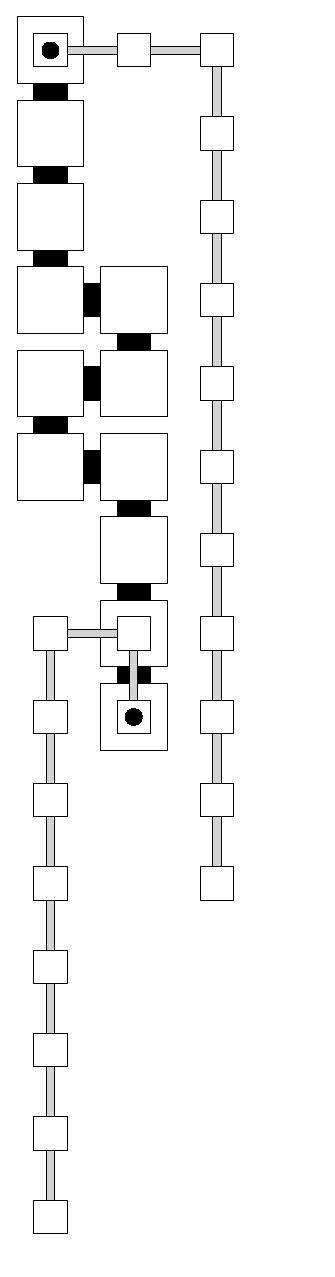
\includegraphics[width=0.32\textwidth]{digit_top_general_topper}
        \caption{\label{fig:topper_gen} General topper}
    \end{subfigure}%
    ~
    \begin{subfigure}[t]{0.32\textwidth}
        \centering
        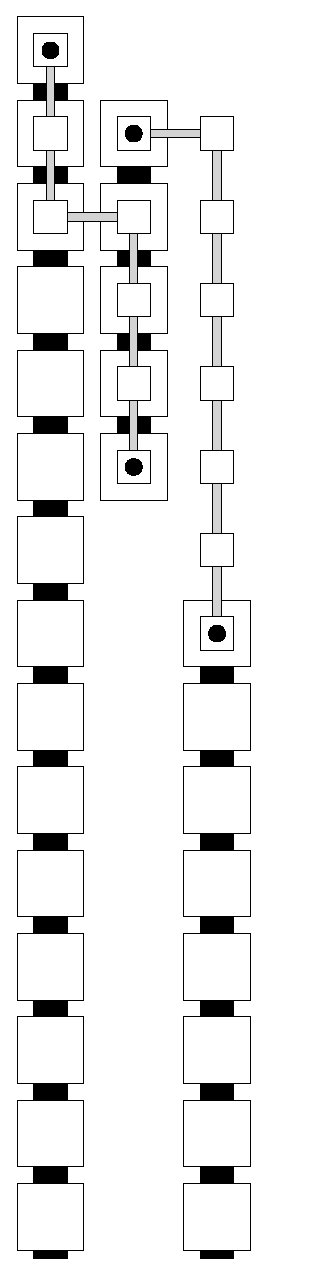
\includegraphics[width=0.32\textwidth]{digit_top_case1_digit1_topper}
        \caption{\label{fig:topper_case1} Case 1 -- topper}
    \end{subfigure}%
    ~
    \begin{subfigure}[t]{0.32\textwidth}
        \centering
        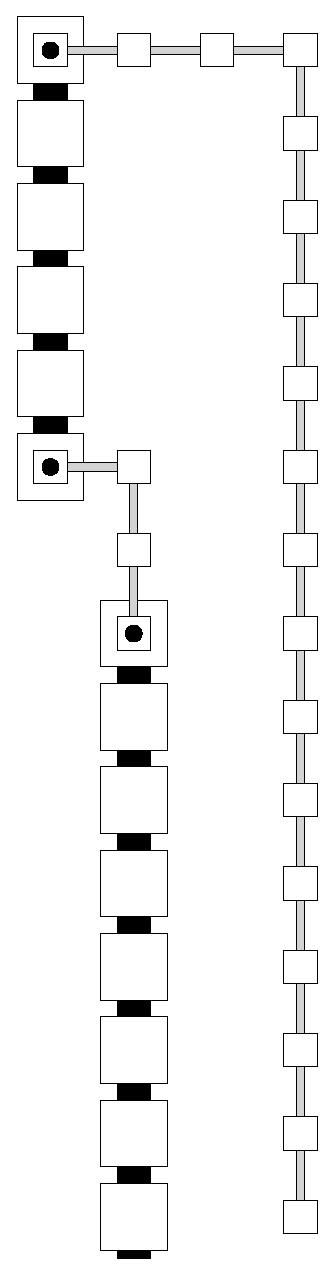
\includegraphics[width=0.32\textwidth]{digit_top_case2_digit2_topper}
        \caption{\label{fig:topper_case2} Case 2 -- topper}
    \end{subfigure}%
    \caption{\label{fig:topper_microgadgets} Topper micro-gadgets }
\end{figure}


    For each $\inc \in \{ {\tt increment, copy } \}$
    \begin{itemize}

        \item Digit 1 (general): the following statements create the gadget shown in Figure~\ref{fig:digit_top_general}.
        \begin{itemize}
            \item Create
            $\begin{aligned}[t]
                {\tt North\_Line5}(& \left \langle {\tt DigitTop},  1, \inc \right\rangle,
                                     \left \langle {\tt DigitTopA}, 1, \inc \right\rangle \;)
            \end{aligned}$\\from the micro-gadget shown in Figure~\ref{fig:north_line}.

            \item Create
            $\begin{aligned}[t]
                {\tt Topper}(& \left \langle {\tt DigitTopA}, 1, \inc \right\rangle,
                               \left \langle {\tt DigitTopB}, 1, \inc \right\rangle \;)
            \end{aligned}$\\from the micro-gadget shown in Figure~\ref{fig:topper_gen}.

            \item Create
            $\begin{aligned}[t]
                {\tt South\_Line4\textit{l}}(& \left\langle {\tt DigitTopB}, 1, \inc \right\rangle,
                                               \left\langle \returnpath,     1, \inc \right\rangle \;)
            \end{aligned}$\\from the micro-gadget shown in Figure~\ref{fig:south_line}.
        \end{itemize}
        %
        In this step, $2 \cdot \left( 40 + 4l \right) =$
        %
        $80 + 8l =$
        %
        $80 + 8 \cdot \left( \ceil*{\log m} + 2 \right) \leq$
        %
        $80 + 8 \cdot \left( {\log m} + 3 \right) =$
        %
        $104 + 8 \cdot {\log m} = \bigologm$ tiles were created.
        %
        \vspace{0.5cm}


        \item Digit 1 (MSR): the following statements create the gadget shown in Figure~\ref{fig:digit_top_1_op_msr}.
        \begin{itemize}
            \item Create
            $\begin{aligned}[t]
                {\tt Topper}(& \left\langle {\tt DigitTop},  1, \inc, {\tt msr} \right\rangle,
                               \left\langle {\tt DigitTopA}, 1, \inc, {\tt msr} \right\rangle \;)
            \end{aligned}$ \\ from the micro-gadget shown in Figure~\ref{fig:topper_case1}.


            \item Create
            $\begin{aligned}[t]
                {\tt South\_Line4\textit{l}}(& \left\langle {\tt DigitTopA}, 1, \inc, {\tt msr}\right\rangle,
                                               \left\langle \returnpath,     1, \inc, {\tt msr}\right\rangle \;)
            \end{aligned}$ \\ from the micro-gadget shown in Figure~\ref{fig:south_line}.
        \end{itemize}
        %
        In this step, $2 \cdot \left( 43 + 4l \right) =$
        %
        $86 + 8l =$
        %
        $86 + 8 \cdot \left( \ceil*{\log m} + 2 \right) \leq$
        %
        $86 + 8 \cdot \left( {\log m} + 3 \right) =$
        %
        $110 + 8 \cdot {\log m} = \bigologm$ tiles were created.
        %
        \vspace{0.5cm}


        \item Digit 1 (MSD): the following statements create the gadget shown in Figure~\ref{fig:digit_top_1_op_msr_msd}.
        \begin{itemize}
            \item Create
            $\begin{aligned}[t]
                {\tt North\_Line4\textit{l}}(& \left\langle {\tt DigitTop},  1, \inc, {\tt msr}, {\tt msd}\right\rangle,
                                               \left\langle {\tt DigitTopA}, 1, \inc, {\tt msr}, {\tt msd}\right\rangle \;)
            \end{aligned}$\\from the micro-gadget shown in Figure~\ref{fig:north_line}.

            \item Create $\begin{aligned}[t]
                {\tt North\_Line4}(& \left\langle {\tt DigitTopA}, 1, \inc, {\tt msr}, {\tt msd}\right\rangle,
                                     \left\langle {\tt DigitTopB}, 1, \inc, {\tt msr}, {\tt msd}\right\rangle \;)
            \end{aligned}$\\from the micro-gadget shown in Figure~\ref{fig:north_line}.

            \item Create $\begin{aligned}[t]
                {\tt Topper}(& \left\langle {\tt DigitTopB}, 1, \inc, {\tt msr}, {\tt msd}\right\rangle,
                               \left\langle {\tt DigitTopC}, 1, \inc, {\tt msr}, {\tt msd}\right\rangle \;)
            \end{aligned}$\\from the micro-gadget shown in Figure~\ref{fig:topper_gen}.

            \item Create
            $\begin{aligned}[t]
                {\tt South\_Line4\textit{l}}(& \left\langle {\tt DigitTopC}, 1, \inc, {\tt msr}, {\tt msd}\right\rangle,
                                               \left\langle {\tt DigitTopD}, 1, \inc, {\tt msr}, {\tt msd}\right\rangle \;)
            \end{aligned}$\\from the micro-gadget shown in Figure~\ref{fig:south_line}.

            \item Create
            $\begin{aligned}[t]
                {\tt South\_Line30}(& \left\langle {\tt DigitTopD}, 1, \inc, {\tt msr}, {\tt msd}\right\rangle,
                                      \left\langle {\tt DigitTopE}, 1, \inc, {\tt msr}, {\tt msd}\right\rangle \;)
            \end{aligned}$\\from the micro-gadget shown in Figure~\ref{fig:south_line}.

            \item Create
            $\begin{aligned}[t]
                {\tt South\_Line4\textit{l}}(& \left\langle {\tt DigitTopE}, 1, \inc, {\tt msr}, {\tt msd}\right\rangle,
                                               \left\langle {\tt DigitTopF}, 1, \inc, {\tt msr}, {\tt msd}\right\rangle \;)
            \end{aligned}$\\ from the micro-gadget shown in Figure~\ref{fig:south_line}.

            \item Create
            $\begin{aligned}[t]
                {\tt South\_Line14}(& \left\langle {\tt DigitTopF}, 1, \inc, {\tt msr}, {\tt msd}\right\rangle,
                                      \left\langle {\tt DigitTopG}, 1, \inc, {\tt msr}, {\tt msd}\right\rangle \;)
            \end{aligned}$\\ from the micro-gadget shown in Figure~\ref{fig:south_line}.

            \item Create
            $\begin{aligned}[t]
                {\tt South\_Line17}(& \left\langle {\tt DigitTopG}, 1, \inc, {\tt msr}, {\tt msd} \right\rangle,
                                      \left\langle \returnpath,     1, \inc, {\tt msr}, {\tt msd} \right\rangle \;)
            \end{aligned}$\\from the micro-gadget shown in Figure~\ref{fig:south_line}.
        \end{itemize}
        %
        In this step, $2 \cdot \left( 100 + 12l \right) =$
        %
        $200 + 24l =$
        %
        $200 + 24 \cdot \left( \ceil*{\log m} + 2 \right) \leq$
        %
        $200 + 24 \cdot \left( {\log m} + 3 \right) =$
        %
        $272 + 24 \cdot {\log m} = \bigologm$ tiles were created.
        %
        \vspace{0.5cm}


        \item Digit 2 (general): the following statements create the gadget shown in Figure~\ref{fig:digit_top_general}.
        \begin{itemize}
            \item Create
            $\begin{aligned}[t]
                {\tt North\_Line5}(& \left\langle {\tt DigitTop}, 2, \inc \right\rangle,
                                     \left\langle {\tt DigitTopA} 2, \inc \right\rangle \;)
            \end{aligned}$\\from the micro-gadget shown in Figure~\ref{fig:north_line}.

            \item Create
            $\begin{aligned}[t]
                {\tt Topper}(& \left\langle {\tt DigitTopA} 2, \inc \right\rangle,
                               \left\langle {\tt DigitTopB} 2, \inc \right\rangle \;)
            \end{aligned}$\\from the micro-gadget shown in Figure~\ref{fig:topper_gen}.

            \item Create
            $\begin{aligned}[t]
                {\tt South\_Line4\textit{l}}(& \left\langle {\tt DigitTopB} 2, \inc \right\rangle,
                                               \left\langle \returnpath,    2, \inc \right\rangle \;)
            \end{aligned}$\\from the micro-gadget shown in Figure~\ref{fig:south_line}.
        \end{itemize}
        %
        In this step $2 \cdot \left( 40 + 4l \right) =$
        %
        $80 + 8l =$
        %
        $80 + 8 \cdot \left( \ceil*{\log m} + 2 \right) \leq$
        %
        $80 + 8 \cdot \left( {\log m} + 3 \right) =$
        %
        $104 + 8 \cdot {\log m} = \bigologm$ tiles were created.
        %
        \vspace{0.5cm}


        \item Digit 2 (MSD): the following statements create the gadget shown in Figure~\ref{fig:digit_top_2_op_msr_msd}.
        \begin{itemize}
            \item Create
            $\begin{aligned}[t]
                {\tt North\_Line4\textit{l}}(& \left\langle {\tt DigitTop},  2, \inc, {\tt msr}, {\tt msd} \right\rangle,
                                               \left\langle {\tt DigitTopA}, 2, \inc, {\tt msr}, {\tt msd} \right\rangle\;)
            \end{aligned}$\\ from the micro-gadget shown in Figure~\ref{fig:north_line}.

            \item Create
            $\begin{aligned}[t]
                {\tt Topper}(& \left\langle {\tt DigitTopA}, 2, \inc, {\tt msr}, {\tt msd} \right\rangle,
                               \left\langle {\tt DigitTopB}, 2, \inc, {\tt msr}, {\tt msd} \right\rangle \;)
            \end{aligned}$\\from the micro-gadget shown in Figure~\ref{fig:topper_case2}.

            \item Create
            $\begin{aligned}[t]
                {\tt South\_Line4\textit{l}}(& \left\langle {\tt DigitTopB}, 2, \inc, {\tt msr}, {\tt msd} \right\rangle,
                                               \left\langle {\tt DigitTopC}, 2, \inc, {\tt msr}, {\tt msd} \right\rangle \;)
            \end{aligned}$\\from the micro-gadget shown in Figure~\ref{fig:south_line}.

            \item Create
            $\begin{aligned}[t]
                {\tt South\_Line30}(& \left\langle {\tt DigitTopC}, 2, \inc, {\tt msr}, {\tt msd} \right\rangle,
                                      \left\langle \returnpath,     2, \inc, {\tt msr}, {\tt msd}\right\rangle \;)
            \end{aligned}$\\from the micro-gadget shown in Figure~\ref{fig:south_line}.
        \end{itemize}
        %
        In this step, $2 \cdot \left( 58 + 8l \right) =$
        %
        $116 + 16l =$
        %
        $116 + 16 \cdot \left( \ceil*{\log m} + 2 \right) \leq$
        %
        $116 + 16 \cdot \left( {\log m} + 3 \right) =$
        %
        $164 + 16 \cdot {\log m} = \bigologm$ tiles were created.
        %
        \vspace{0.5cm}


        \item Digit 3 (general): the following statements create the gadget from Figure~\ref{fig:digit_top_general}.
        \begin{itemize}
            \item Create
            $\begin{aligned}[t]
                {\tt North\_Line5}(& \left\langle {\tt DigitTop},  3, \inc \right\rangle,
                                     \left\langle {\tt DigitTopA}, 3, \inc \right\rangle \;)
            \end{aligned}$\\from the micro-gadget shown in Figure~\ref{fig:north_line}.

            \item Create
            $\begin{aligned}[t]
                {\tt Topper}(& \left\langle {\tt DigitTopA}, 3, \inc  \right\rangle,
                               \left\langle {\tt DigitTopB}, 3, \inc  \right\rangle \;)
            \end{aligned}$\\from the micro-gadget shown in Figure~\ref{fig:topper_gen}.

            \item Create
            $\begin{aligned}[t]
                {\tt South\_Line4\textit{l}}(& \left\langle {\tt DigitTopB}, 3, \inc \right\rangle,
                                               \left\langle \returnpath,     3, \inc \right\rangle \;)
            \end{aligned}$\\from the micro-gadget shown in Figure~\ref{fig:south_line}.
        \end{itemize}
        %
        In this step, $2 \cdot \left( 40 + 4l \right) =$
        %
        $80 + 8l =$
        %
        $80 + 8 \cdot \left( \ceil*{\log m} + 2 \right) \leq$
        %
        $80 + 8 \cdot \left( {\log m} + 3 \right) =$
        %
        $104 + 8 \cdot {\log m} = \bigologm$ tiles were created.
        %
        \vspace{0.5cm}


        \item Digit 3 (MSD): the following statements create the gadget from Figure~\ref{fig:digit_top_general}.
        \begin{itemize}
            \item Create
            $\begin{aligned}[t]
                {\tt North\_Line5}(& \left\langle {\tt DigitTop},  3, \inc, {\tt msr}, {\tt msd}\right\rangle,
                                     \left\langle {\tt DigitTopA}, 3, \inc, {\tt msr}, {\tt msd}\right\rangle \;)
            \end{aligned}$\\from the micro-gadget shown in Figure~\ref{fig:north_line}.

            \item Create
            $\begin{aligned}[t]
                {\tt Topper}(& \left\langle {\tt DigitTopA}, 3, \inc, {\tt msr}, {\tt msd}\right\rangle,
                               \left\langle {\tt DigitTopB}, 3, \inc, {\tt msr}, {\tt msd}\right\rangle \;)
            \end{aligned}$\\ from the micro-gadget shown in Figure~\ref{fig:topper_gen}.


            \item Create
            $\begin{aligned}[t]
                {\tt South\_Line4\textit{l}}(& \left\langle {\tt DigitTopB}, 3, \inc, {\tt msr}, {\tt msd}\right\rangle,
                                               \left\langle \returnpath,     3, \inc, {\tt msr}, {\tt msd}\right\rangle \;)
            \end{aligned}$\\ from the micro-gadget shown in Figure~\ref{fig:south_line}.
        \end{itemize}
        %
        In this step, $2 \cdot \left( 40 + 4l \right) =$
        %
        $80 + 8l =$
        %
        $80 + 8 \cdot \left( \ceil*{\log m} + 2 \right) \leq$
        %
        $80 + 8 \cdot \left( {\log m} + 3 \right) =$
        %
        $104 + 8 \cdot {\log m} = \bigologm$ tiles were created.
        %
    \end{itemize}

    \begin{figure}[H]
        \centering
        \subcaptionbox{
            Digits 1, 2, \& 3 - general.
            \label{fig:digit_top_general}
        }{\makebox[0.24\textwidth][c]{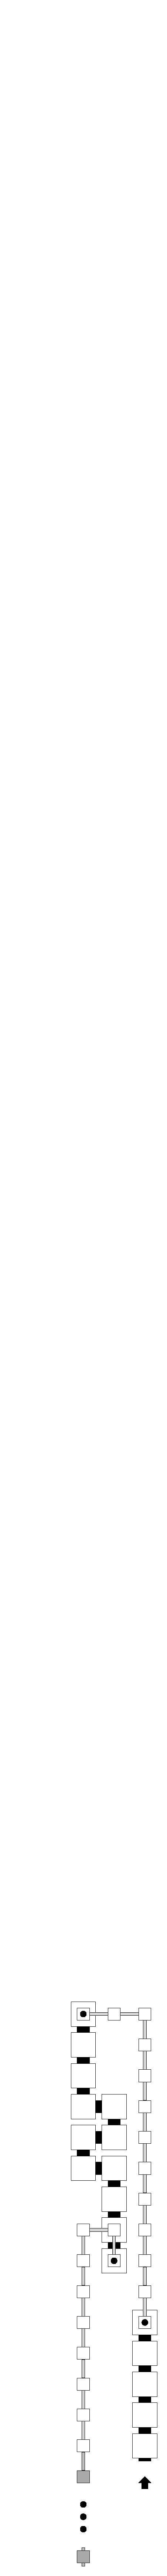
\includegraphics[width=0.45in]{digit_top_general}}}%
        ~
        \subcaptionbox{
            Digit 1 - general\\ overview.
            The black tiles in this figure correspond to the gadget shown in subfigure~\subref{fig:digit_top_general}.
            \label{fig:digit_top_1_op_overview}
        }{\makebox[0.24\textwidth][c]{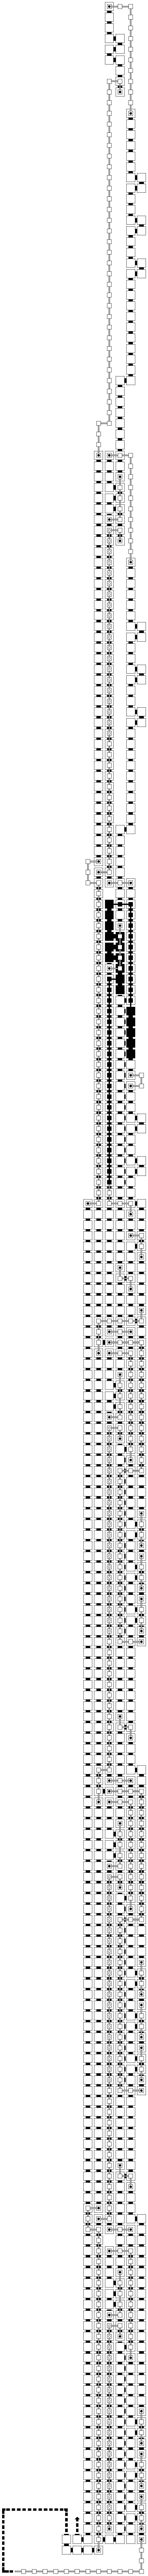
\includegraphics[width=0.45in]{overviews/general/digit_top_1_op}}}%
        ~
        \subcaptionbox{
            Digit 1 - general (seed) overview.
            The black tiles in this figure correspond to the gadget shown in subfigure~\subref{fig:digit_top_general}.
            \label{fig:digit_top_1_seed_op_overview}
        }{\makebox[0.24\textwidth][c]{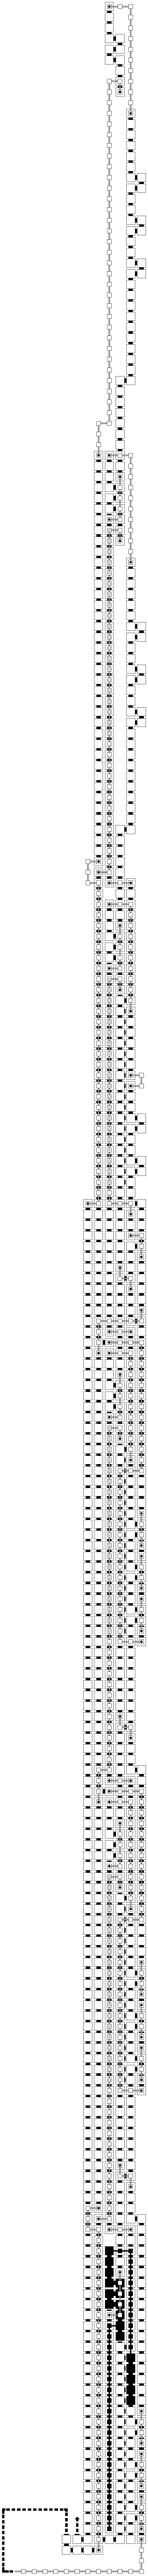
\includegraphics[width=0.45in]{overviews/general/digit_top_1_seed_op}}}%
        ~
        \subcaptionbox{
            Digit 2 - general\\ overview.
            The black tiles in this figure correspond to the gadget shown in subfigure~\subref{fig:digit_top_general}.
            \label{fig:digit_top_2_op_overview}
        }{\makebox[0.24\textwidth][c]{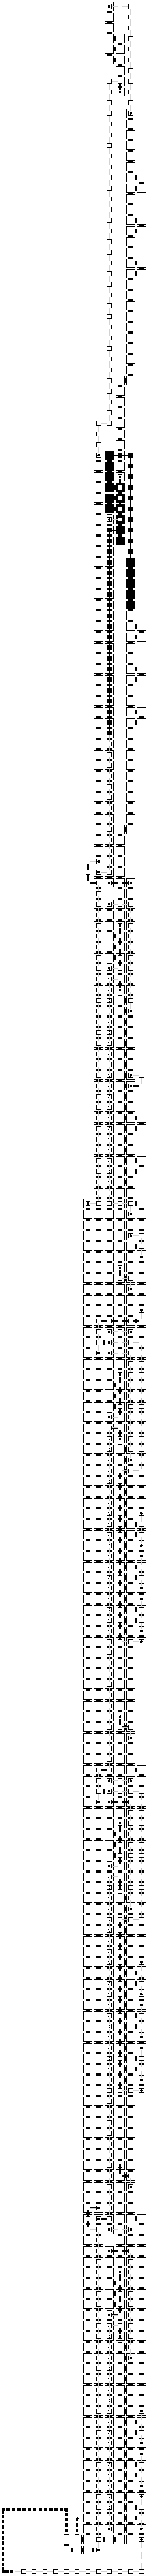
\includegraphics[width=0.45in]{overviews/general/digit_top_2_op}}}%
        ~
    \end{figure}
    \begin{figure}[H]\ContinuedFloat
        \centering
        \subcaptionbox{
            Digit 2 - general (seed) overview.
            The black tiles in this figure correspond to the gadget shown in subfigure~\subref{fig:digit_top_general}.
            \label{fig:digit_top_2_seed_op_overview}
        }{\makebox[0.24\textwidth][c]{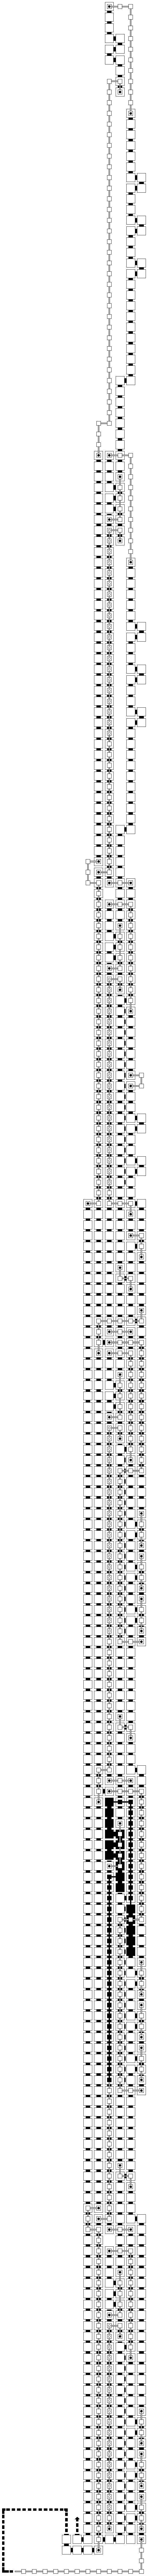
\includegraphics[width=0.45in]{overviews/general/digit_top_2_seed_op}}}%
        ~
        \subcaptionbox{
            Digit 3 - general\\ overview.
            The black tiles in this figure correspond to the gadget shown in subfigure~\subref{fig:digit_top_general}.
            \label{fig:digit_top_3_op_overview}
        }{\makebox[0.24\textwidth][c]{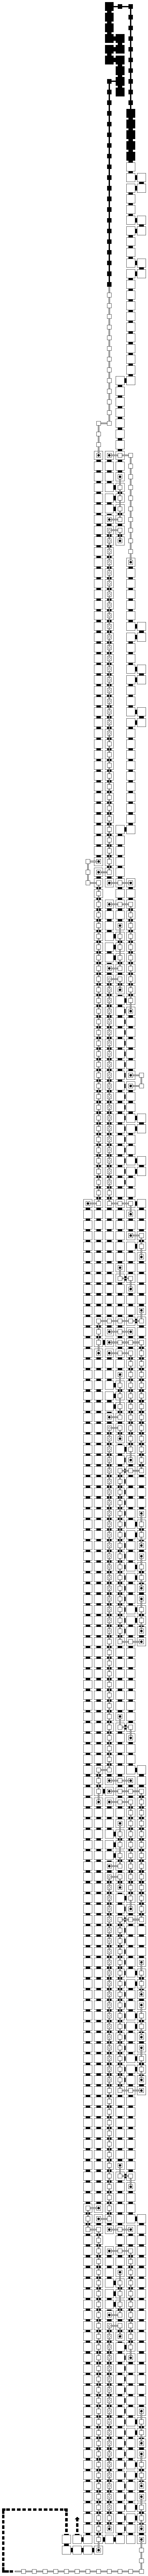
\includegraphics[width=0.45in]{overviews/general/digit_top_3_op}}}%
        ~
        \subcaptionbox{
            Digit 3 - general (seed) overview.
            The black tiles in this figure correspond to the gadget shown in subfigure~\subref{fig:digit_top_general}.
            \label{fig:digit_top_3_seed_op_overview}
        }{\makebox[0.24\textwidth][c]{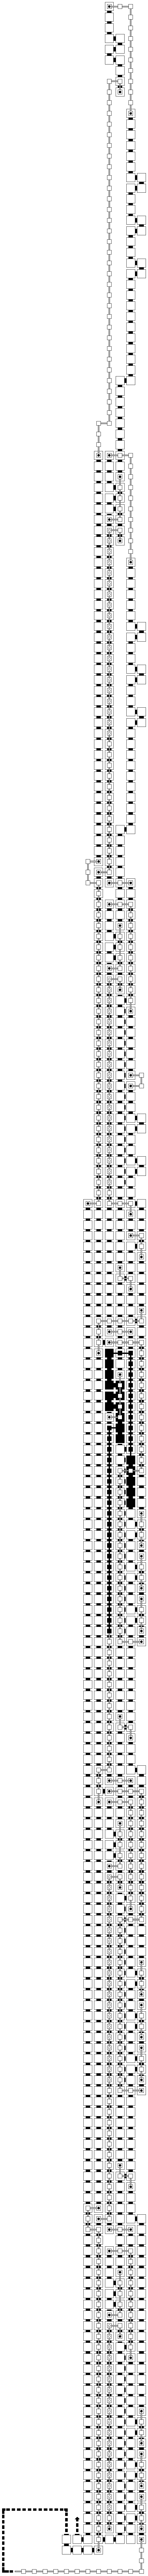
\includegraphics[width=0.45in]{overviews/general/digit_top_3_seed_op}}}%
        ~
        \subcaptionbox{
            Digit 1 - case 1.
            \label{fig:digit_top_1_op_msr_msd}
        }{\makebox[0.24\textwidth][c]{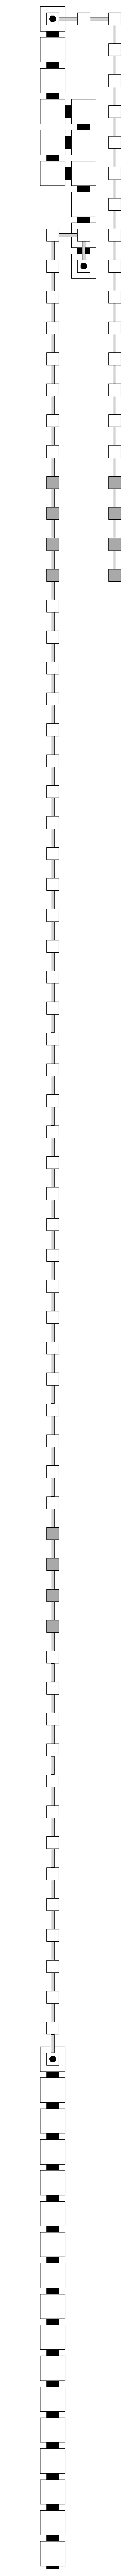
\includegraphics[width=0.45in]{digit_top_case1_digit1_msr}}}%
        ~
    \end{figure}
    \begin{figure}[H]\ContinuedFloat
        \centering
        \subcaptionbox{
            Digit 1 - case 1 overview.
            The black tiles in this figure correspond to the gadget shown in subfigure~\subref{fig:digit_top_1_op_msr_msd}.
            \label{fig:digit_top_1_op_msr_msd_overview}
        }{\makebox[0.24\textwidth][c]{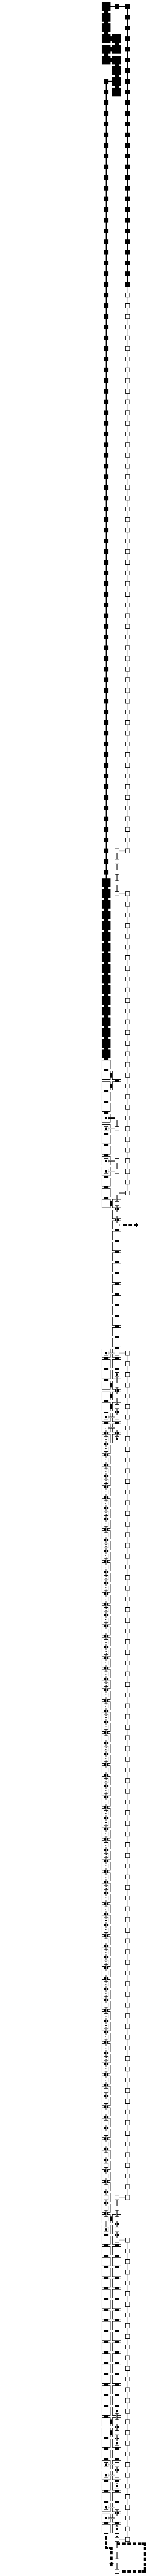
\includegraphics[width=0.45in]{overviews/case1/digit_top_1_op_msr_msd}}}%
        ~
        \subcaptionbox{
            Digit 1 - case 1 (seed) overview.
            The black tiles in this figure correspond to the gadget shown in subfigure~\subref{fig:digit_top_1_op_msr_msd}.
            \label{fig:digit_top_1_seed_op_msr_msd_overview}
        }{\makebox[0.24\textwidth][c]{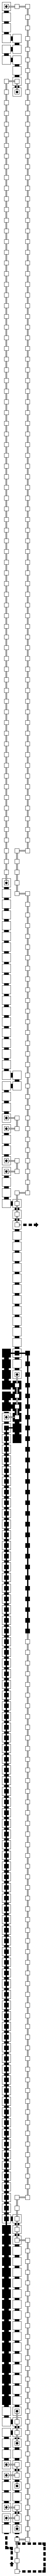
\includegraphics[width=0.45in]{overviews/case1/digit_top_1_seed_op_msr_msd}}}%
        ~
        \subcaptionbox{
            Digit 1 - case 2.
            \label{fig:digit_top_1_op_msr}
        }{\makebox[0.24\textwidth][c]{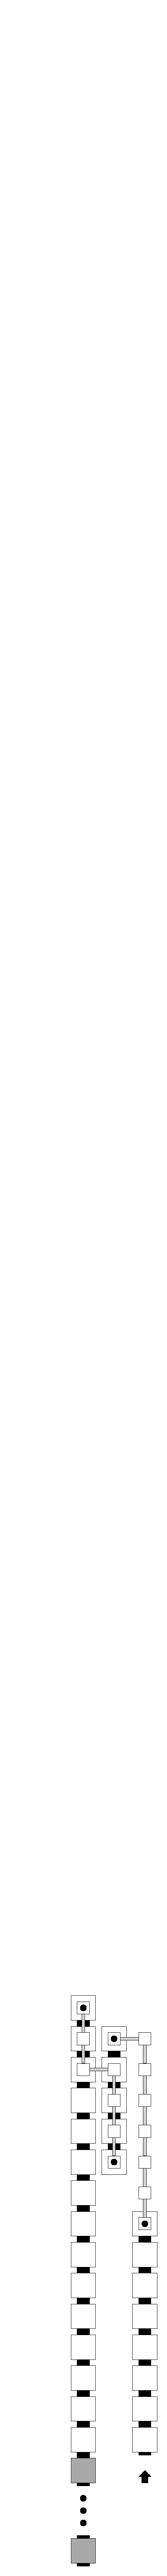
\includegraphics[width=0.45in]{digit_top_case2_digit1_msr}}}%
        ~
        \subcaptionbox{
            Digit 1 - case 2 overview.
            The black tiles in this figure correspond to the gadget shown in subfigure~\subref{fig:digit_top_1_op_msr}.
            \label{fig:digit_top_1_op_msr_overview}
        }{\makebox[0.24\textwidth][c]{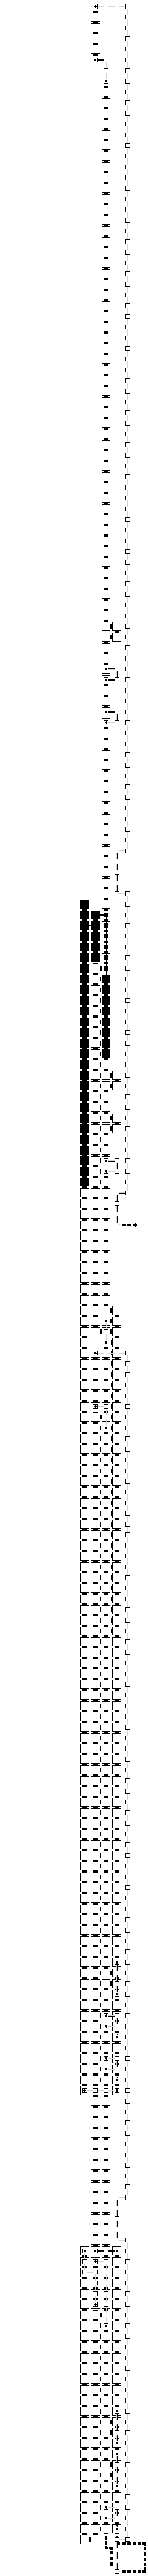
\includegraphics[width=0.45in]{overviews/case2/digit_top_1_op_msr}}}%
        ~
    \end{figure}
    \begin{figure}[H]\ContinuedFloat
        \centering
        \subcaptionbox{
            Digit 1 - case 2 (seed) overview.
            The black tiles in this figure correspond to the gadget shown in subfigure~\subref{fig:digit_top_1_op_msr}.
            \label{fig:digit_top_1_seed_op_msr_overview}
        }{\makebox[0.24\textwidth][c]{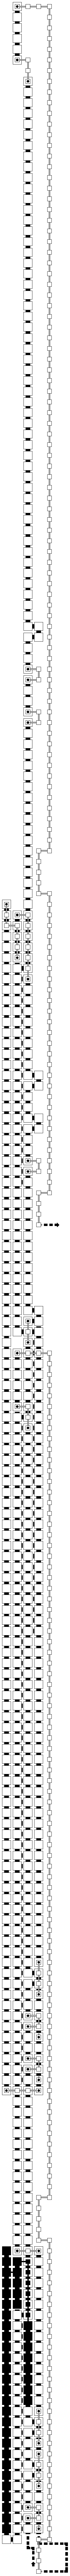
\includegraphics[width=0.45in]{overviews/case2/digit_top_1_seed_op_msr}}}%
        ~
        \subcaptionbox{
            Digit 2 - case 2.
            \label{fig:digit_top_2_op_msr_msd}
        }{\makebox[0.24\textwidth][c]{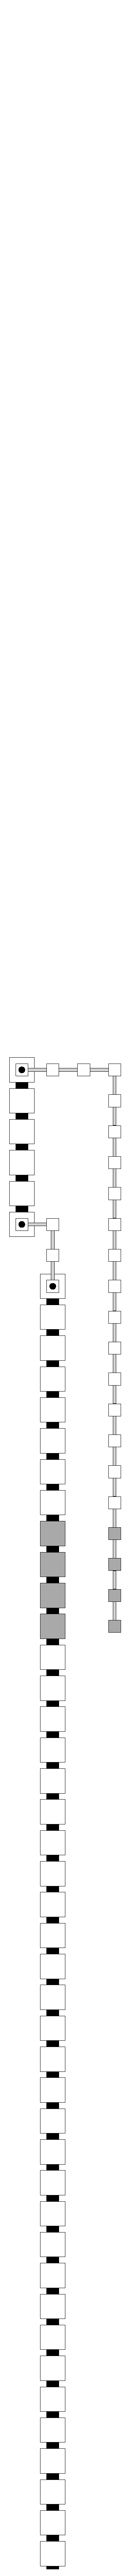
\includegraphics[width=0.45in]{digit_top_case2_digit2_msr}}}%
        ~
        \subcaptionbox{
            Digit 2 - case 2 overview.
            The black tiles in this figure correspond to the gadget shown in subfigure~\subref{fig:digit_top_2_op_msr_msd}.
            \label{fig:digit_top_2_op_msr_msd_overview}
        }{\makebox[0.24\textwidth][c]{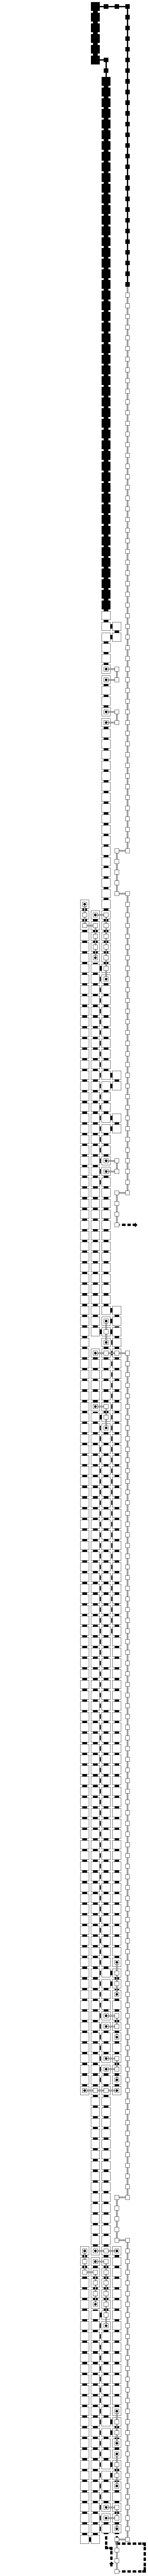
\includegraphics[width=0.45in]{overviews/case2/digit_top_2_op_msr_msd}}}%
        ~
        \subcaptionbox{
            Digit 2 - case 2 (seed) overview.
            The black tiles in this figure correspond to the gadget shown in subfigure~\subref{fig:digit_top_2_op_msr_msd}.
            \label{fig:digit_top_2_seed_op_msr_msd_overview}
        }{\makebox[0.24\textwidth][c]{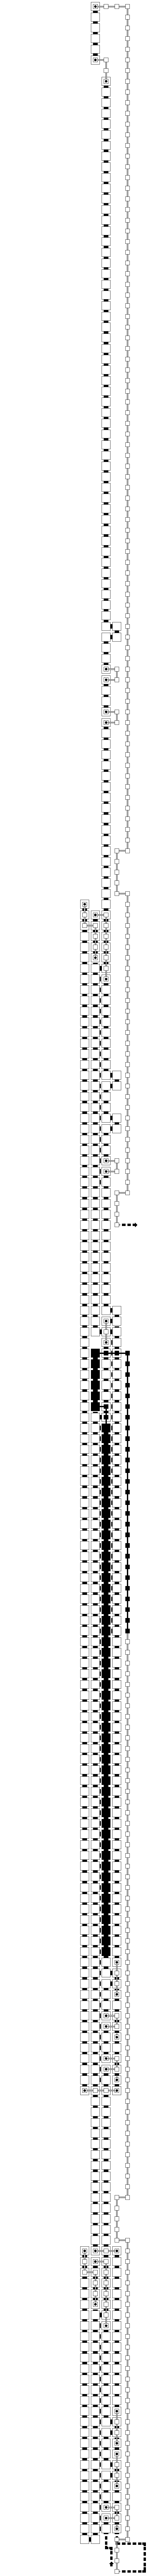
\includegraphics[width=0.45in]{overviews/case2/digit_top_2_seed_op_msr_msd}}}%
        ~
    \end{figure}
    \begin{figure}[H]\ContinuedFloat
        \centering
        \subcaptionbox{
            Digit 3 - case 3.
            \label{fig:digit_top_3_op_msr_msd}
        }{\makebox[0.24\textwidth][c]{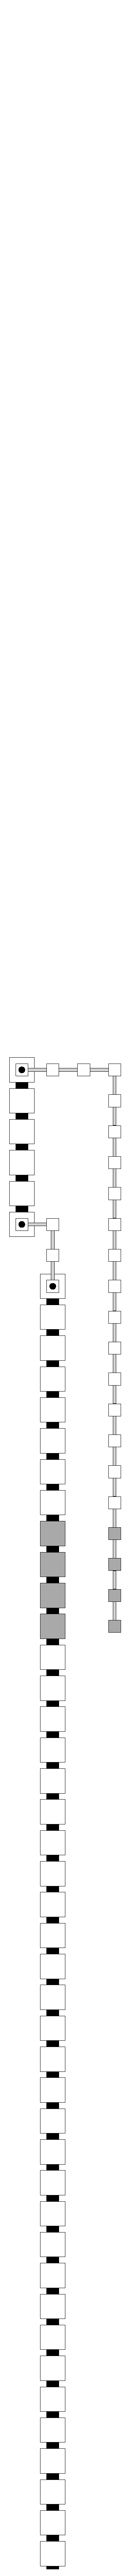
\includegraphics[width=0.33in]{digit_top_case2_digit2_msr}}}%
        ~
        \subcaptionbox{
            Digit 3 - case 3 overview.
            The black tiles in this figure correspond to the gadget shown in subfigure~\subref{fig:digit_top_3_op_msr_msd}.
            \label{fig:digit_top_3_op_msr_msd_overview}
        }{\makebox[0.24\textwidth][c]{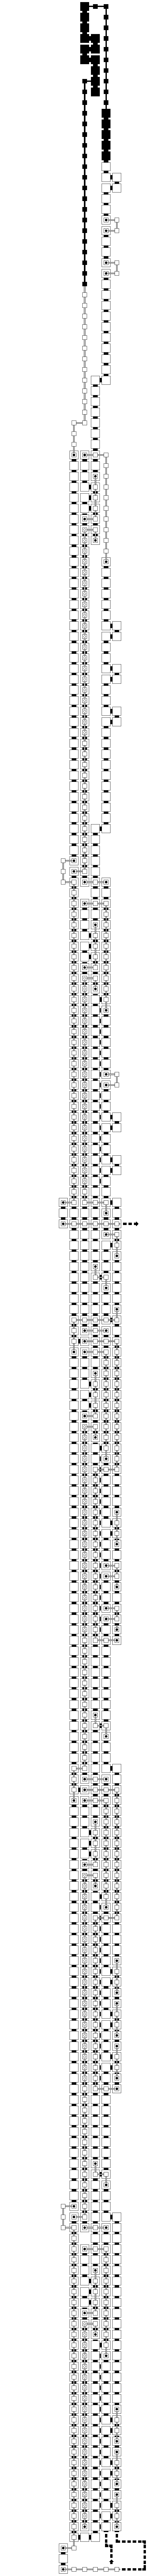
\includegraphics[width=0.45in]{overviews/case3/digit_top_3_op_msr_msd}}}%
        ~
        \subcaptionbox{
            Digit 3 - case 3 (seed) overview.
            The black tiles in this figure correspond to the gadget shown in subfigure~\subref{fig:digit_top_3_op_msr_msd}.
            \label{fig:digit_top_3_seed_op_msr_msd_overview}
        }{\makebox[0.24\textwidth][c]{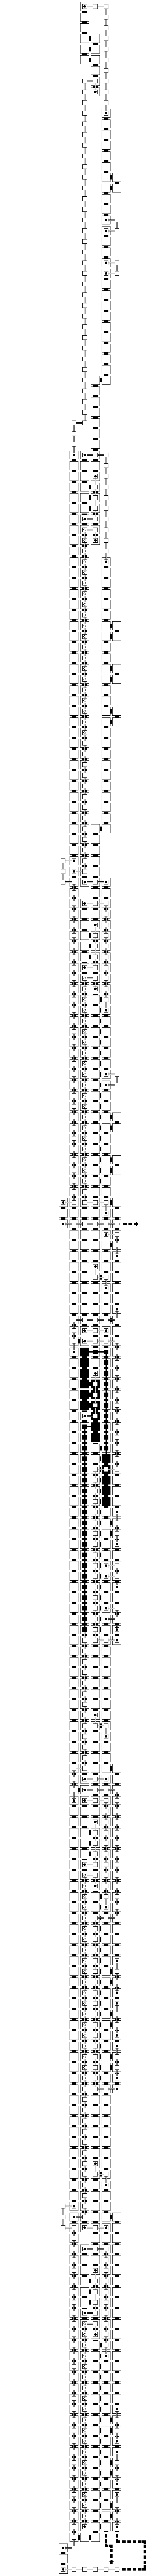
\includegraphics[width=0.45in]{overviews/case3/digit_top_3_seed_op_msr_msd}}}%
        ~
        \caption{\label{fig:digit_tops} The {\tt Digit\_Top} gadgets.}
    \end{figure}

\vspace{1cm}
